\documentclass{article}
\usepackage{longtable}
\usepackage{tabu}
\usepackage{lscape}
\usepackage{float}
\usepackage{adjustbox}
\usepackage{Sweave}
\begin{document}
\Sconcordance{concordance:WC86R1.tex:WC86R1.Rnw:%
1 6 1 1 0 14 1 1 2 1 0 2 1 3 0 2 2 4 0 2 2 1 0 5 1 3 0 2 2 1 0 1 1 3 0 %
2 2 4 0 2 2 6 0 2 1 6 0 1 2 1 1 1 2 1 0 1 1 3 0 2 2 6 0 2 1 6 0 2 2 6 0 %
2 1 6 0 2 2 4 0 1 2 2 1 1 4 1 2 5 1 1 2 8 0 1 2 3 1 1 3 1 2 5 1 1 2 4 0 %
1 2 1 1 1 2 4 0 1 2 3 1 1 2 1 0 1 2 6 0 1 4 1 5 4 0 1 5 3 0 1 5 7 0 1 3 %
1 5 4 0 1 5 3 0 1 5 8 0 1 4 1 5 4 0 1 5 3 0 1 4 8 0 1 4 1 5 4 0 1 5 3 0 %
1 4 6 0 1 2 1 10 12 0 2 2 1 0 1 1 3 0 2 2 4 0 1 2 1 1 1 2 4 0 1 2 1 1 1 %
2 1 0 1 4 6 0 2 2 4 0 1 2 1 1 1 4 19 0 1 2 4 1 1 13 1 2 8 1 1 13 1 2 9 %
1 1 13 1 2 7 1}


\title{Analysis of wallaby and kangaroo line transect data}
\author{David L. Borchers and Martin J. Cox}
\maketitle
\section{Summary}
\begin{enumerate}
\item I am a little concerned that I have missed something by not scaling the positions in the previous analysis, so I am going to do so here.
\end{enumerate}

\section{Overview}
This analysis is confined to examining the wallaby sighting line transect data where the transects were orientated North-South.  I selected the North-South direction because the transect lengths were similar and the range of transect observation durations, no worse than the East-West transect durations. 

\subsection{User defined variables}
\begin{Schunk}
\begin{Sinput}
> w=160 #m (half inter-transect spacing)
> ystart=400 #m  
> wy=160#20 # y-dimesion truncation distance
\end{Sinput}
\end{Schunk}
I am adding a 'scale factor' to reduce the apparent survey area size in order to better accommodate alternative hazard functions.  I may have missed something here, and this could be complete nonsense, but I thought I'd try it:
\begin{Schunk}
\begin{Sinput}
> scaleFactor=100
\end{Sinput}
\end{Schunk}
Load \texttt{R} packages:
\begin{Schunk}
\begin{Sinput}
> source('~/Dropbox/packages/2D distance sampling with time/R/2DLTfunctions.r')
> library(xlsx)
> library(psych)
> library(xtable)
> library(scatterplot3d)
> library(rgl)
\end{Sinput}
\end{Schunk}
Next we read in sightings and transect data.  To do so, we will need the \texttt{xlsx} package.
\begin{Schunk}
\begin{Sinput}
> transects=read.xlsx('~/Dropbox/packages/2D distance sampling with time/data/landSurveys/WC86TN.xlsx',sheetIndex=1)
> sightings=read.xlsx('~/Dropbox/packages/2D distance sampling with time/data/landSurveys/WC86IS.xlsx',sheetIndex=1)  
\end{Sinput}
\end{Schunk}
Merge the data:
\begin{Schunk}
\begin{Sinput}
> sightings=merge(sightings,transects,'TNNU')
\end{Sinput}
\end{Schunk}
Now we'll subset the data, retaining the wallaby data on North-South transects
\begin{Schunk}
\begin{Sinput}
> nrow(sightings)
\end{Sinput}
\begin{Soutput}
[1] 1124
\end{Soutput}
\begin{Sinput}
> sub=subset(sightings,SPEC=='RNW' & TBRG %in% c(90,270))#c(0,180))## )
> nrow(sub)
\end{Sinput}
\begin{Soutput}
[1] 227
\end{Soutput}
\end{Schunk}
\section{Calculate x,y coordinates}
Calculate x and y coordinates:
\begin{Schunk}
\begin{Sinput}
> sub$X=with(sub,RADL*sin(ANGL*pi/180))
> sub$Y=with(sub,RADL*cos(ANGL*pi/180))
\end{Sinput}
\end{Schunk}
We take \texttt{ANGL} to be a relative bearing to the sighting with 90 deg being abeam or perpendicular to the transect, so we remove sightings where \texttt{ANGL}$>$90 deg:
\begin{Schunk}
\begin{Sinput}
> nrow(sub)
\end{Sinput}
\begin{Soutput}
[1] 227
\end{Soutput}
\begin{Sinput}
> sub=subset(sub,ANGL<=90)
> nrow(sub)
\end{Sinput}
\begin{Soutput}
[1] 202
\end{Soutput}
\end{Schunk}
and subset on truncation distances:
\begin{Schunk}
\begin{Sinput}
> nrow(sub)
\end{Sinput}
\begin{Soutput}
[1] 202
\end{Soutput}
\begin{Sinput}
> sub=subset(sub,X<w & Y<wy)
> nrow(sub)
\end{Sinput}
\begin{Soutput}
[1] 183
\end{Soutput}
\end{Schunk}
Remove non-zero y-distances:
\begin{Schunk}
\begin{Sinput}
> sub$Y[sub$Y<1]=1
\end{Sinput}
\end{Schunk}
We need the transects to be observed at a constant speed so checking transect speed:
\begin{figure}
\begin{center}
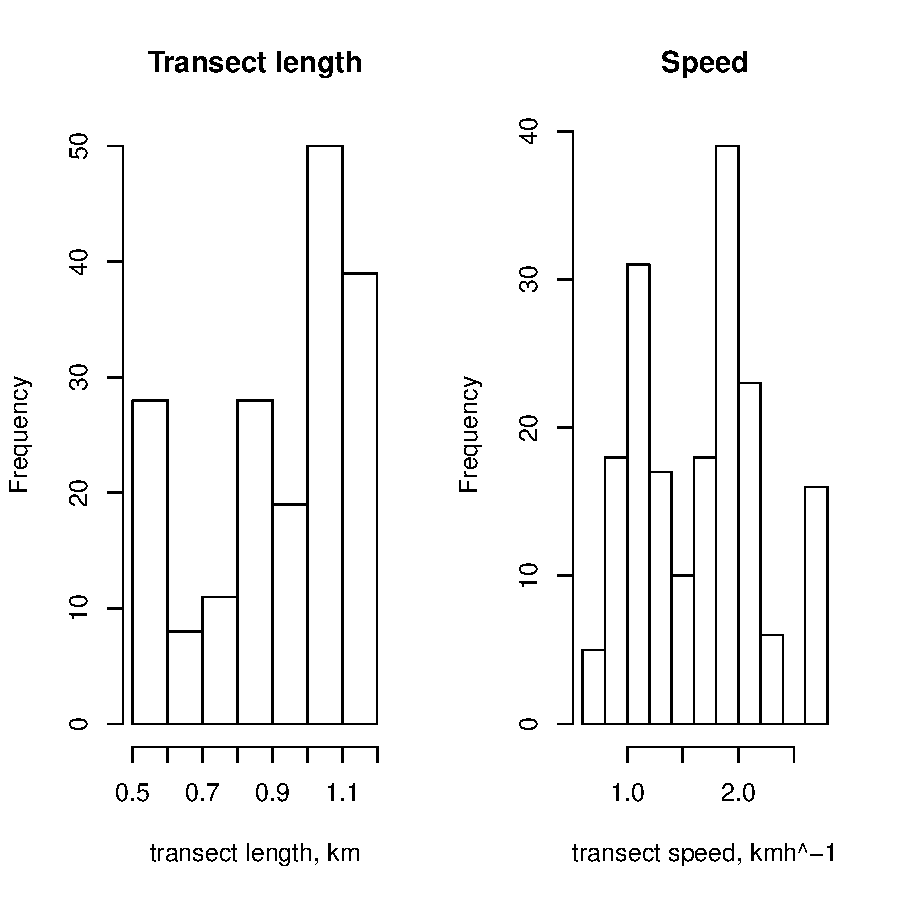
\includegraphics{WC86R1-fig1}
\end{center}
\caption{Transect lengths and survey speeds.}
\label{fig:one}
\end{figure}

and the direction of transects:
\begin{Schunk}
\begin{Sinput}
> table(sub$TBRG)
\end{Sinput}
\begin{Soutput}
 90 270 
100  83 
\end{Soutput}
\end{Schunk}

Display the sightings
\begin{figure}
\begin{center}
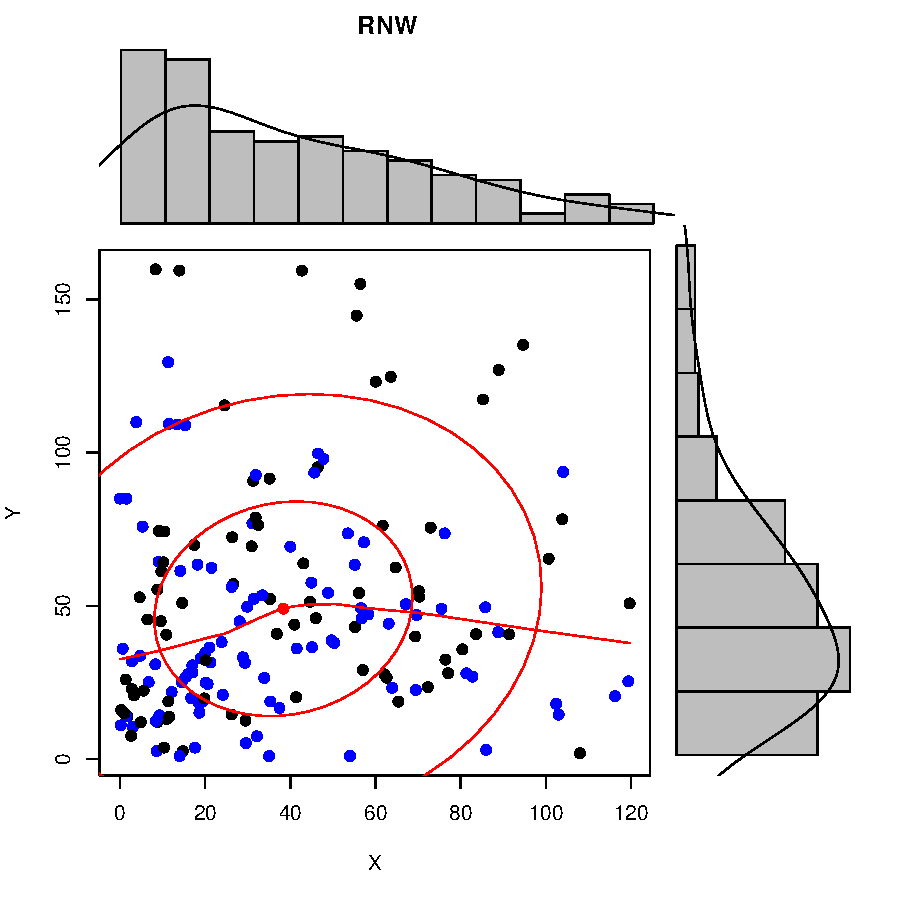
\includegraphics{WC86R1-fig2}
\end{center}
\caption{Observations for wallabys (RNW).}
\label{fig:two}
\end{figure}

\subsection{Group size as a covariate}
\begin{Schunk}
\begin{Sinput}
> with(sub,scatterplot3d(x=X,y=Y,z=GPSZ,color=as.numeric(as.factor(TDRN)),type="h",angle=60))
\end{Sinput}
\end{Schunk}

Also using \texttt{rgl}:
\begin{Schunk}
\begin{Sinput}
> with(sub,plot3d(x=X,y=Y,z=GPSZ,col=as.numeric(as.factor(TDRN)),type="h"))
\end{Sinput}
\end{Schunk}

\subsection{Analysis of the NS and SN wallaby (RNW) sightings}
Models are fit using the wallaby sighting data.  Three perpendicular density functions are considered: (i) uniform; (ii) half-normal, and (iii) normal.  
The models take a while to fit, so the results have been stored in an \texttt{R} workspace:
\begin{Schunk}
\begin{Sinput}
> load('~/Dropbox/packages/2D distance sampling with time/data/landSurveys/workspace.RData')
> #get revised functions:
> source('~/Dropbox/packages/2D distance sampling with time/R/2DLTfunctions.r')
> 
> 
\end{Sinput}
\end{Schunk}

\begin{Schunk}
\begin{Sinput}
> #fit uniform perpendicular density function with h1 hazard function:
> mod1.unif.h1=fityx(y=sub$Y/scaleFactor,x=sub$X/scaleFactor,b=log(c(1,1)),hr=h1,
+                  ystart=ystart/scaleFactor,
+                  pi.x=pi.const,logphi=NULL,w=w/scaleFactor,hessian=TRUE)
> #fit half-normal perpendicular density function with h1 hazard function:
> mod2.hn.h1=fityx(y=sub$Y/scaleFactor,x=sub$X/scaleFactor,b=log(c(1,1)),hr=h1,
+                ystart=ystart/scaleFactor,
+                  pi.x=pi.hnorm,logphi=1,w=w/scaleFactor,hessian=TRUE)
> #normal perpendicular density function with h1 hazard function:
> mod3.n.h1=fityx(y=sub$Y/scaleFactor,x=sub$X/scaleFactor,b=c(-1.65,0.86),hr=h1,
+               ystart=ystart/scaleFactor,
+                  pi.x=pi.norm,logphi=c(0.1,1),w=w/scaleFactor,hessian=TRUE)
> 
\end{Sinput}
\end{Schunk}
Now models are fit using the \texttt{h2} hazard function:
\begin{Schunk}
\begin{Sinput}
> #fit uniform perpendicular density function with h2 hazard function:
> mod4.unif.h2=fityx(y=sub$Y/scaleFactor,x=sub$X/scaleFactor,b=log(c(0.75,1)),hr=h2,
+                  ystart=ystart/scaleFactor,
+                  pi.x=pi.const,logphi=NULL,w=w/scaleFactor,hessian=TRUE)
> #fit half-normal perpendicular density function with h2 hazard function:
> mod5.hn.h2=fityx(y=sub$Y/scaleFactor,x=sub$X/scaleFactor,b=c(-1.9,-0.48),hr=h2,
+                ystart=ystart/scaleFactor,
+                  pi.x=pi.hnorm,logphi=2,w=w/scaleFactor,hessian=TRUE)
> #normal perpendicular density function with h2 hazard function:
> mod6.n.h2=fityx(y=sub$Y/scaleFactor,x=sub$X/scaleFactor,b=c(-1.9,-0.48),hr=h2,
+               ystart=ystart/scaleFactor,
+                  pi.x=pi.norm,logphi=c(0.1,1),w=w/scaleFactor,hessian=TRUE)
> 
> 
\end{Sinput}
\end{Schunk}
Using the Okamura et al. (2003) hazard function:
\begin{Schunk}
\begin{Sinput}
> #fit uniform perpendicular density function with the h.okamura hazard function:
> mod7.unif.h.okamura=fityx(y=sub$Y/scaleFactor,x=sub$X/scaleFactor,b=log(c(0.75,1)),hr=h.okamura,
+                  ystart=ystart/scaleFactor,
+                  pi.x=pi.const,logphi=NULL,w=w/scaleFactor,hessian=TRUE)
> #fit half-normal perpendicular density function with the h.okamura hazard function:
> mod8.hn.h.okamura=fityx(y=sub$Y/scaleFactor,x=sub$X/scaleFactor,b=c(-0.93,-0.77),hr=h.okamura,
+                ystart=ystart/scaleFactor,
+                  pi.x=pi.hnorm,logphi=1,w=w/scaleFactor,hessian=TRUE)
> #fit a normal perpendicular density function with the h.okamura hazard function:
> mod9.n.h.okamura=fityx(y=sub$Y/scaleFactor,x=sub$X/scaleFactor,b=c(-0.93,-0.77),hr=h.okamura,
+                ystart=ystart/scaleFactor,
+                  pi.x=pi.norm,logphi=c(1,1),w=w/scaleFactor,hessian=TRUE)
> 
> 
\end{Sinput}
\end{Schunk}
Also fit with the exponential power hazard model of Skaug \& Schweder 1999:
\begin{Schunk}
\begin{Sinput}
> #fit uniform perpendicular density function with the Exponential power hazard model of Skaug & Schweder 1999 for the hazard function:
> mod10.unif.h.exp=fityx(y=sub$Y/scaleFactor,x=sub$X/scaleFactor,b=log(c(0.75,0.9)),hr=h.exp2,
+                  ystart=ystart/scaleFactor,
+                  pi.x=pi.const,logphi=NULL,w=w/scaleFactor,hessian=TRUE)
> #fit half-normal perpendicular density function with the Exponential power hazard model of Skaug & Schweder 1999 for the hazard function:
> mod11.hn.h.exp=fityx(y=sub$Y/scaleFactor,x=sub$X/scaleFactor,b=c(-1.77,-0.26),hr=h.exp2,
+                ystart=ystart/scaleFactor,
+                  pi.x=pi.hnorm,logphi=7,w=w/scaleFactor,hessian=TRUE)
> #fit a normal perpendicular density function with the Exponential power hazard model of Skaug & Schweder 1999 for the hazard function:
> mod12.n.h.exp=fityx(y=sub$Y/scaleFactor,x=sub$X/scaleFactor,b=c(-1.77,-0.26),hr=h.exp2,
+                ystart=ystart/scaleFactor,
+                  pi.x=pi.norm,logphi=c(1,1),w=w/scaleFactor,hessian=TRUE)
\end{Sinput}
\end{Schunk}
Create a list of models:
\begin{Schunk}
\begin{Sinput}
> modL=list(h1.unif=mod1.unif.h1,h1.hn=mod2.hn.h1,
+           h1.n=mod3.n.h1,
+                       h2.unif=mod4.unif.h2,h2.hn=mod5.hn.h2,h2.norm=mod6.n.h2,
+                       h.okamura.unif=mod7.unif.h.okamura,
+                       h.okamura.hn=mod8.hn.h.okamura,
+                       h.okamura.norm=mod9.n.h.okamura,
+                       h.exp.unif=mod10.unif.h.exp,
+                       h.exp.hn=mod11.hn.h.exp,
+                       h.exp.n=mod12.n.h.exp)
\end{Sinput}
\end{Schunk}
Remove models with fit errors:
\begin{Schunk}
\begin{Sinput}
> me=sapply(modL,function(x) x$error)
> modLR=modL[!me]
\end{Sinput}
\end{Schunk}
I am suspicous of the Okamura hazard rate models, I wonder if these models have got stuck at a local minima.  Perhaps using different starting parameter values could check this.  For now, I will remove the Okamura models:
\begin{Schunk}
\begin{Sinput}
> modLR=modLR[-grep('okamura',names(modLR))]
\end{Sinput}
\end{Schunk}
AIC-based model selection was carried out using the \texttt{modSelect} function:

\begin{Schunk}
\begin{Sinput}
> aicTab=modSelect(modLR,modNames=names(modLR),tab=TRUE)
\end{Sinput}
\end{Schunk}
Estimate $\hat{p}$ with confidence intervals obtained using the delta method as well as $\hat{N}$:

\begin{Schunk}
\begin{Sinput}
> phatTab=phatModels(modList=modLR[aicTab$AICorder],n=nrow(sub),tab=TRUE)
> tab1=xtable(cbind(aicTab$tab,phatTab$tab),label='tab:model.sel',
+             caption='AIC-based model selection for the various combinations of hazard and 
+             perpendicular density functions. n is the number of parameters.  () is the coefficient
+             of variation, or for Nhat is the 95 confidence interval.')
\end{Sinput}
\end{Schunk}
Order models by AIC:
\begin{Schunk}
\begin{Sinput}
> modLR=modLR[aicTab$AICorder]
\end{Sinput}
\end{Schunk}
\begin{landscape}
\begin{small}
% latex table generated in R 3.1.2 by xtable 1.7-4 package
% Sun Jan 11 07:48:56 2015
{\small
\begin{longtable}{rllrrrrrll}
\caption{AIC-based model selection for the various combinations of hazard and 
            perpendicular density functions. n is the number of parameters.  () is the coefficient
            of variation, or for Nhat is the 95 confidence interval.} \\ 
  \hline
 & bhat & logphihat & n & logLik & AIC & dAIC & w & phat & Nhat \\ 
  \hline
h1.n & -1.77(0.09); 0.88(0.05) & 0.43(0.23); -0.64(0.28) & 4.00 & 59.39 & 122.79 & 0.00 & 0.81 & 0.46(0.12) & 394(313,497) \\ 
  h1.hn & -1.65(0.08); 0.86(0.05) & 0.86(0.16); NA(NA) & 3.00 & 61.36 & 125.72 & 2.93 & 0.19 & 0.51(0.1) & 362(297,441) \\ 
  h1.unif & -1.92(0.07); 0.94(0.04) & NA(NA); NA(NA) & 2.00 & 66.85 & 135.70 & 12.91 & 0.00 & 0.35(0.06) & 525(469,588) \\ 
  h2.norm & -2.3(0.09); -0.27(0.6) & 0.7(0.09); -0.88(0.14) & 4.00 & 66.07 & 136.14 & 13.36 & 0.00 & 0.18(0.21) & 999(662,1507) \\ 
  h2.unif & -1.86(0.07); -0.48(0.31) & NA(NA); NA(NA) & 2.00 & 78.01 & 158.01 & 35.23 & 0.00 & 0.26(0.06) & 694(619,777) \\ 
  h2.hn & -1.81(0.08); -0.53(0.34) & 2.14(0.95); NA(NA) & 3.00 & 77.86 & 158.73 & 35.94 & 0.00 & 0.29(0.16) & 640(473,867) \\ 
   \hline
\hline
\label{tab:model.sel}
\end{longtable}
}\end{small}
\end{landscape}
\clearpage
\begin{figure}
\begin{center}
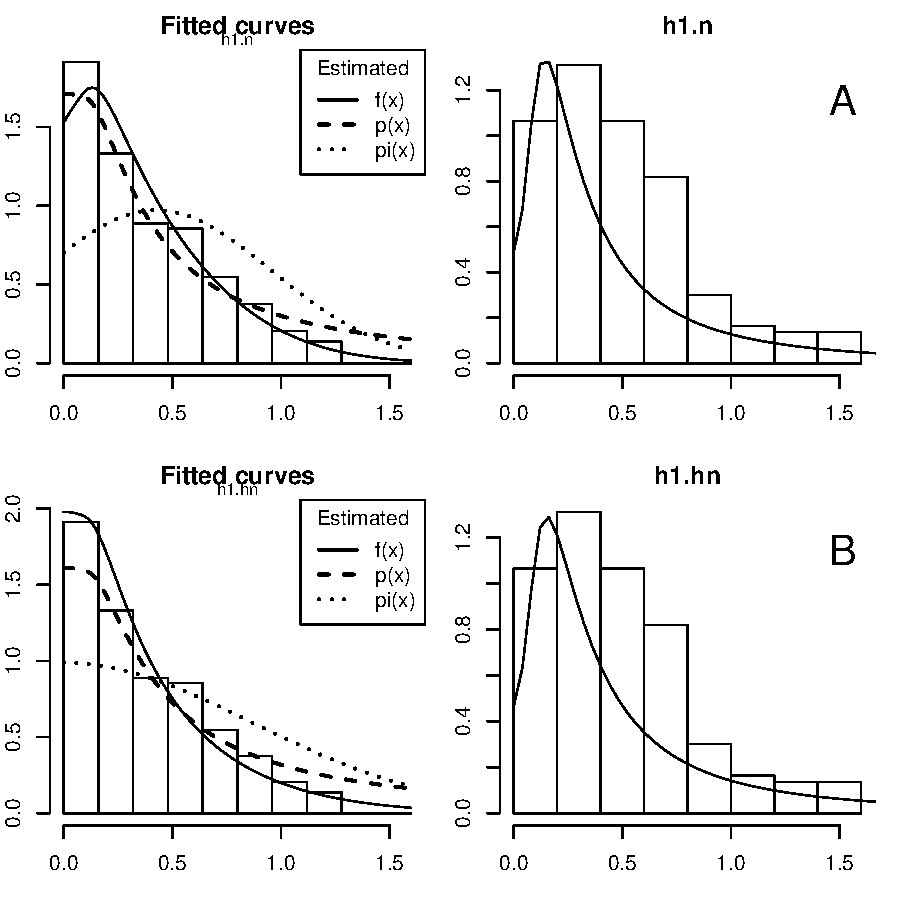
\includegraphics{WC86R1-figmod1}
\end{center}
\caption{Model results for the h1 hazard rate function with a normal perpendicular density distribution (row A) and 
half-normal (row B). LH column is perpendicular distance, x-dimension, and RH column is forward distance, y-dimension. }
\label{fig:mod1and2}
\end{figure}
\clearpage

\begin{figure}
\begin{center}
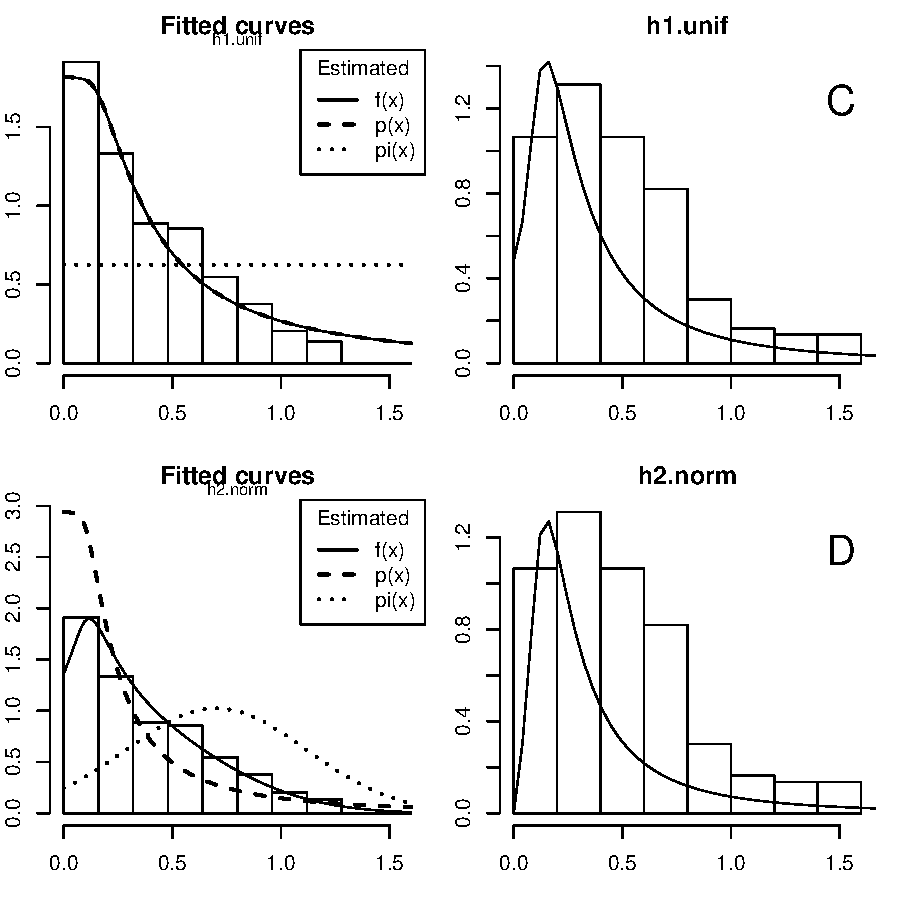
\includegraphics{WC86R1-figmod2}
\end{center}
\caption{Model results for the h1 hazard rate function with a uniform perpendicular density distribution (row C) and 
h2 hazard rate function with a normal perpendicular density distribution(row D).LH column is perpendicular distance, x-dimension, and RH column is forward distance, y-dimension.}
\label{fig:mod3and4}
\end{figure}
\clearpage


\begin{figure}
\begin{center}
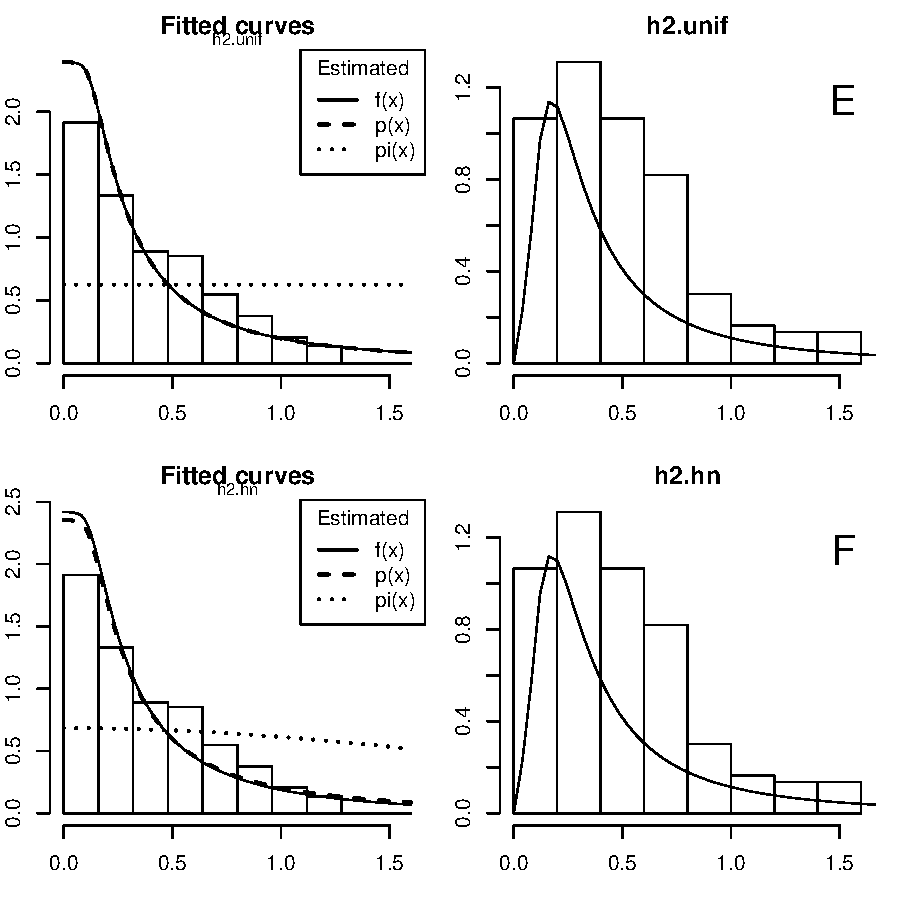
\includegraphics{WC86R1-figmod3}
\end{center}
\caption{Model results for the h2 hazard rate function with a uniform perpendicular density distribution (row E) and a half-normal perpendicular density distribution (row F). LH column is perpendicular distance, x-dimension, and RH column is forward distance, y-dimension.}
\label{fig:mod5and6}
\end{figure}
\clearpage

\end{document}

